\documentclass[11pt,a4paper,twoside]{article}

% ===============================
% Encoding and fonts
% ===============================
\usepackage[T1]{fontenc}
\usepackage{lmodern}

% ===============================
% Page layout
% ===============================
\usepackage[a4paper,margin=2.5cm]{geometry}

% ===============================
% Math
% ===============================
\usepackage{amsmath,amssymb}

% ===============================
% Figures
% ===============================
\usepackage{graphicx}
\usepackage{float}
\usepackage{caption}
\usepackage{subcaption}

% ===============================
% Tables
% ===============================
\usepackage{booktabs}

% ===============================
% Formatting
% ===============================
\usepackage{parskip}   % no paragraph indentation
\usepackage{setspace}
\onehalfspacing

% ===============================
% Utilities
% ===============================
\usepackage{placeins}  % for \FloatBarrier

% ===============================
% Hyperlinks (must be late)
% ===============================
\usepackage[hidelinks]{hyperref}

% ===============================
% References
% ===============================
\usepackage[backend=biber,style=numeric,sorting=none]{biblatex}
\addbibresource{references.bib}



% ===============================
% Document
% ===============================

\begin{document}

\title{Agent-Based Monte Carlo Simulation of Tumor Growth}
\author{Lubna Al-Rifaie, Sabina Saleem and Suraiya Yesmin jakiya}
\date{\today}

\maketitle

% ===============================
\section{Introduction}

In-silico simulations are becoming increasingly used to study cancer biology, as they enable the combined effects of multiple biological
and physical factors to be investigated within a controlled framework, thereby improving our ability to understand and predict tumor behavior\cite{Wang2014}.
This is particularly relevant for solid tumors, where spatial constraints, local cell–cell interactions, and stochastic effects play an 
important role in shaping growth dynamics.

In this context, agent-based models (ABMs) have been widely applied to simulate and study tumor growth. A common formulation employs 
on-lattice models, where cells occupy sites on a regular grid and interact with neighboring cells. In cancer growth modeling, ABMs 
are well suited to capture spatial heterogeneity and emergent behavior arising from cell–cell interactions and environmental constraints\cite{Drasdo2005} \cite{Chkhaidze2019}.

In thisproject, tumor growth is modeled using an agent-based Monte Carlo approach, an approach that has been used in previous studies
to simulate multicellular tumor growth \cite{RuizArrebola2020}. The aim of this work is to develop a model that can be used to study the impact of
stochasticity, spatial constraints and oxygen availability on tumor growth within growing healthy cell population. The stochastic
nature of cellular processes is simulated using Monte Carlo methods implemented in the Julia programming language, in which events 
such as division, death, clearance of dead cells, and mutation-site occur probabilistically at each time step.


\section{Model and Methods}

The tumor is simulated on a two-dimensional square lattice of size $N \times N$, where in this work $N=301$. 
Each lattice site can be empty or occupied by a normal cell, a cancer cell, or a dead cell. The system is 
initialized with a single normal cell placed at the center of the lattice. Time evolution proceeds in discrete 
steps using a Monte Carlo update scheme. At each time step, all living cells are visited once,
and probablistic decisions for division or death are made taking into account the local oxygen availability.


The oxygen field is prescribed as a static, radially symmetric profile that is lowest at the lattice core and
increases toward the lattice boundary, mimicking diffusion-limited oxygen supply. It is defined in Equation~\eqref{eq:oxygen}.

\begin{equation}
O(r) = O_{\min} + \left(1 - O_{\min}\right)\left(1 - e^{-r/L}\right)
\label{eq:oxygen}
\end{equation}

where $r$ is the distance from the lattice center, $O_{\min}$ denotes the minimum oxygen level used in the model, and $L$ controls
the characteristic length scale of oxygen recovery, and in our model it is fixed 

Cell division is attempted by placing a daughter cell in a neighboring empty site. If no empty site is available,
division may still occur through a pushing mechanism, in which a chain of neighboring cells is displaced along 
a lattice direction until an empty site is reached. Cancer cells are assigned a higher probability to push neighboring
cells compared to normal cells, reflecting their enhanced mechanical aggressiveness. For normal cells, the pushing
probability is set to a very small value as shown in Table~\ref{table:parameters} and is therefore negligible in practice. 
Dead cells are removed stochastically with a fixed clearance probability $p_{\text{clear}} = 0.02$, allowing space to be freed up over time.

A former cancer cell occurs by introducing a mutation event in a normal cell that has at least one neighboring empty lattice site. 
The mutation time $t_{\text{mut}}$ can be controlled to explore different growth scenarios, and simulations 
using different random seeds can be used to generate independent realizations of the stochastic process.

Division and death probabilities depend on both the cell type and the local oxygen concentration, with baseline
parameter values summarized in Table~\ref{table:parameters}. Oxygen enters the model as a phenomenological factor 
that biases cell fate toward division in well-oxygenated regions and toward death under hypoxic conditions, as defined in Eq.~\eqref{eq:oxygen_fate}.
Normal cell division is assumed to scale strongly with oxygen availability, whereas cancer cells are allowed
to maintain a finite probability of division even in hypoxic environments. For the results shown here, a minimum oxygen level 
$O_{\min} = 0.35 $ is imposed, which limits the degree of hypoxia experienced by cells. 
This parameter can be varied in future simulations to explore more severe hypoxic conditions.
If neither division nor death occurs during a given time step, the cell remains unchanged.

\begin{table}[H]
\centering
\caption{Effective probabilities used in the simulations.}
\begin{tabular}{lcc}
\toprule
Parameter & Normal cells & Cancer cells \\
\midrule
Push probability $p_{\text{push}}$ & 0.01 & 0.25 \\
Division probability $p_{\text{div}}$ & 0.30 & 0.40 \\
Death probability $p_{\text{death}}$ & 0.05 & 0.02 \\
\bottomrule
\end{tabular}
\label{table:parameters}
\end{table}



\begin{equation}
\begin{aligned}
p_{\mathrm{div}}(O) &=
\begin{cases}
p_{\mathrm{div}}^{N}\, O, \\
p_{\mathrm{div}}^{C}\,(0.5 + 0.5\,O),
\end{cases} \\[6pt]
p_{\mathrm{death}}(O) &=
\begin{cases}
p_{\mathrm{death}}^{N}\,(1 - O), \\
p_{\mathrm{death}}^{C}\,(1 - O),
\end{cases} \\[6pt]
p_{\mathrm{quies}}(O) &= 1 - p_{\mathrm{div}}(O) - p_{\mathrm{death}}(O).
\end{aligned}
\label{eq:oxygen_fate}
\end{equation}

\noindent\textbf{Oxygen-dependent cell fate probabilities.}
Here, $O \in [O_{\min},1]$ denotes the local oxygen concentration, with $O_{\min}=0.35$.
Superscripts $N$ and $C$ refer to normal and cancer cells, respectively.




% ===============================
\section{Results and Discussion}
% ===============================

\subsection{Effect of mutation timing on tumor growth}

In figure~\ref{fig:seed6}, the effect of mutation timing on tumor growth is illustrated for seed 6. 
The left panel shows the lattice snapshot at the mutation time $t = 50,\; 90,\; 150,\; \text{and}\; 200$. 
$O_{2}^{\mathrm{mut}}$is the local oxygen concentration at the mutation site. The former cancer cell is marked by a yellow circle.

These snapshots illustrate how the timing of the mutation influences the spatial competition between cancer and normal cells.
When the mutation occurs at an earlier time, the cancer population has more time to expand, resulting in stronger crowding 
and a clear dominance over the surrounding normal cells. In contrast, for later mutation times, normal cells have already
proliferated and occupied a larger fraction of the lattice before the mutation takes place, leading to a more abundance of normal cells. 

Mutations introduced at early time points ($t= 50, 90, 150$) occure at the periphery, while when it was introduced at ($t = 200$), it occurs at more centrally located 
site. This situation might arise from the stochastic clearance of dead cells implemented in the model, which free up an empty site for cells to divide into, and later
on growth happens through the pushing mechanisim. Cancer growth in this case remains significantly reduced compared to earlier mutation times, highlighting 
the importance of early mutation events and spatial constraint in driving tumor expansion.  

\newpage
\begin{figure}[H]
  \centering
  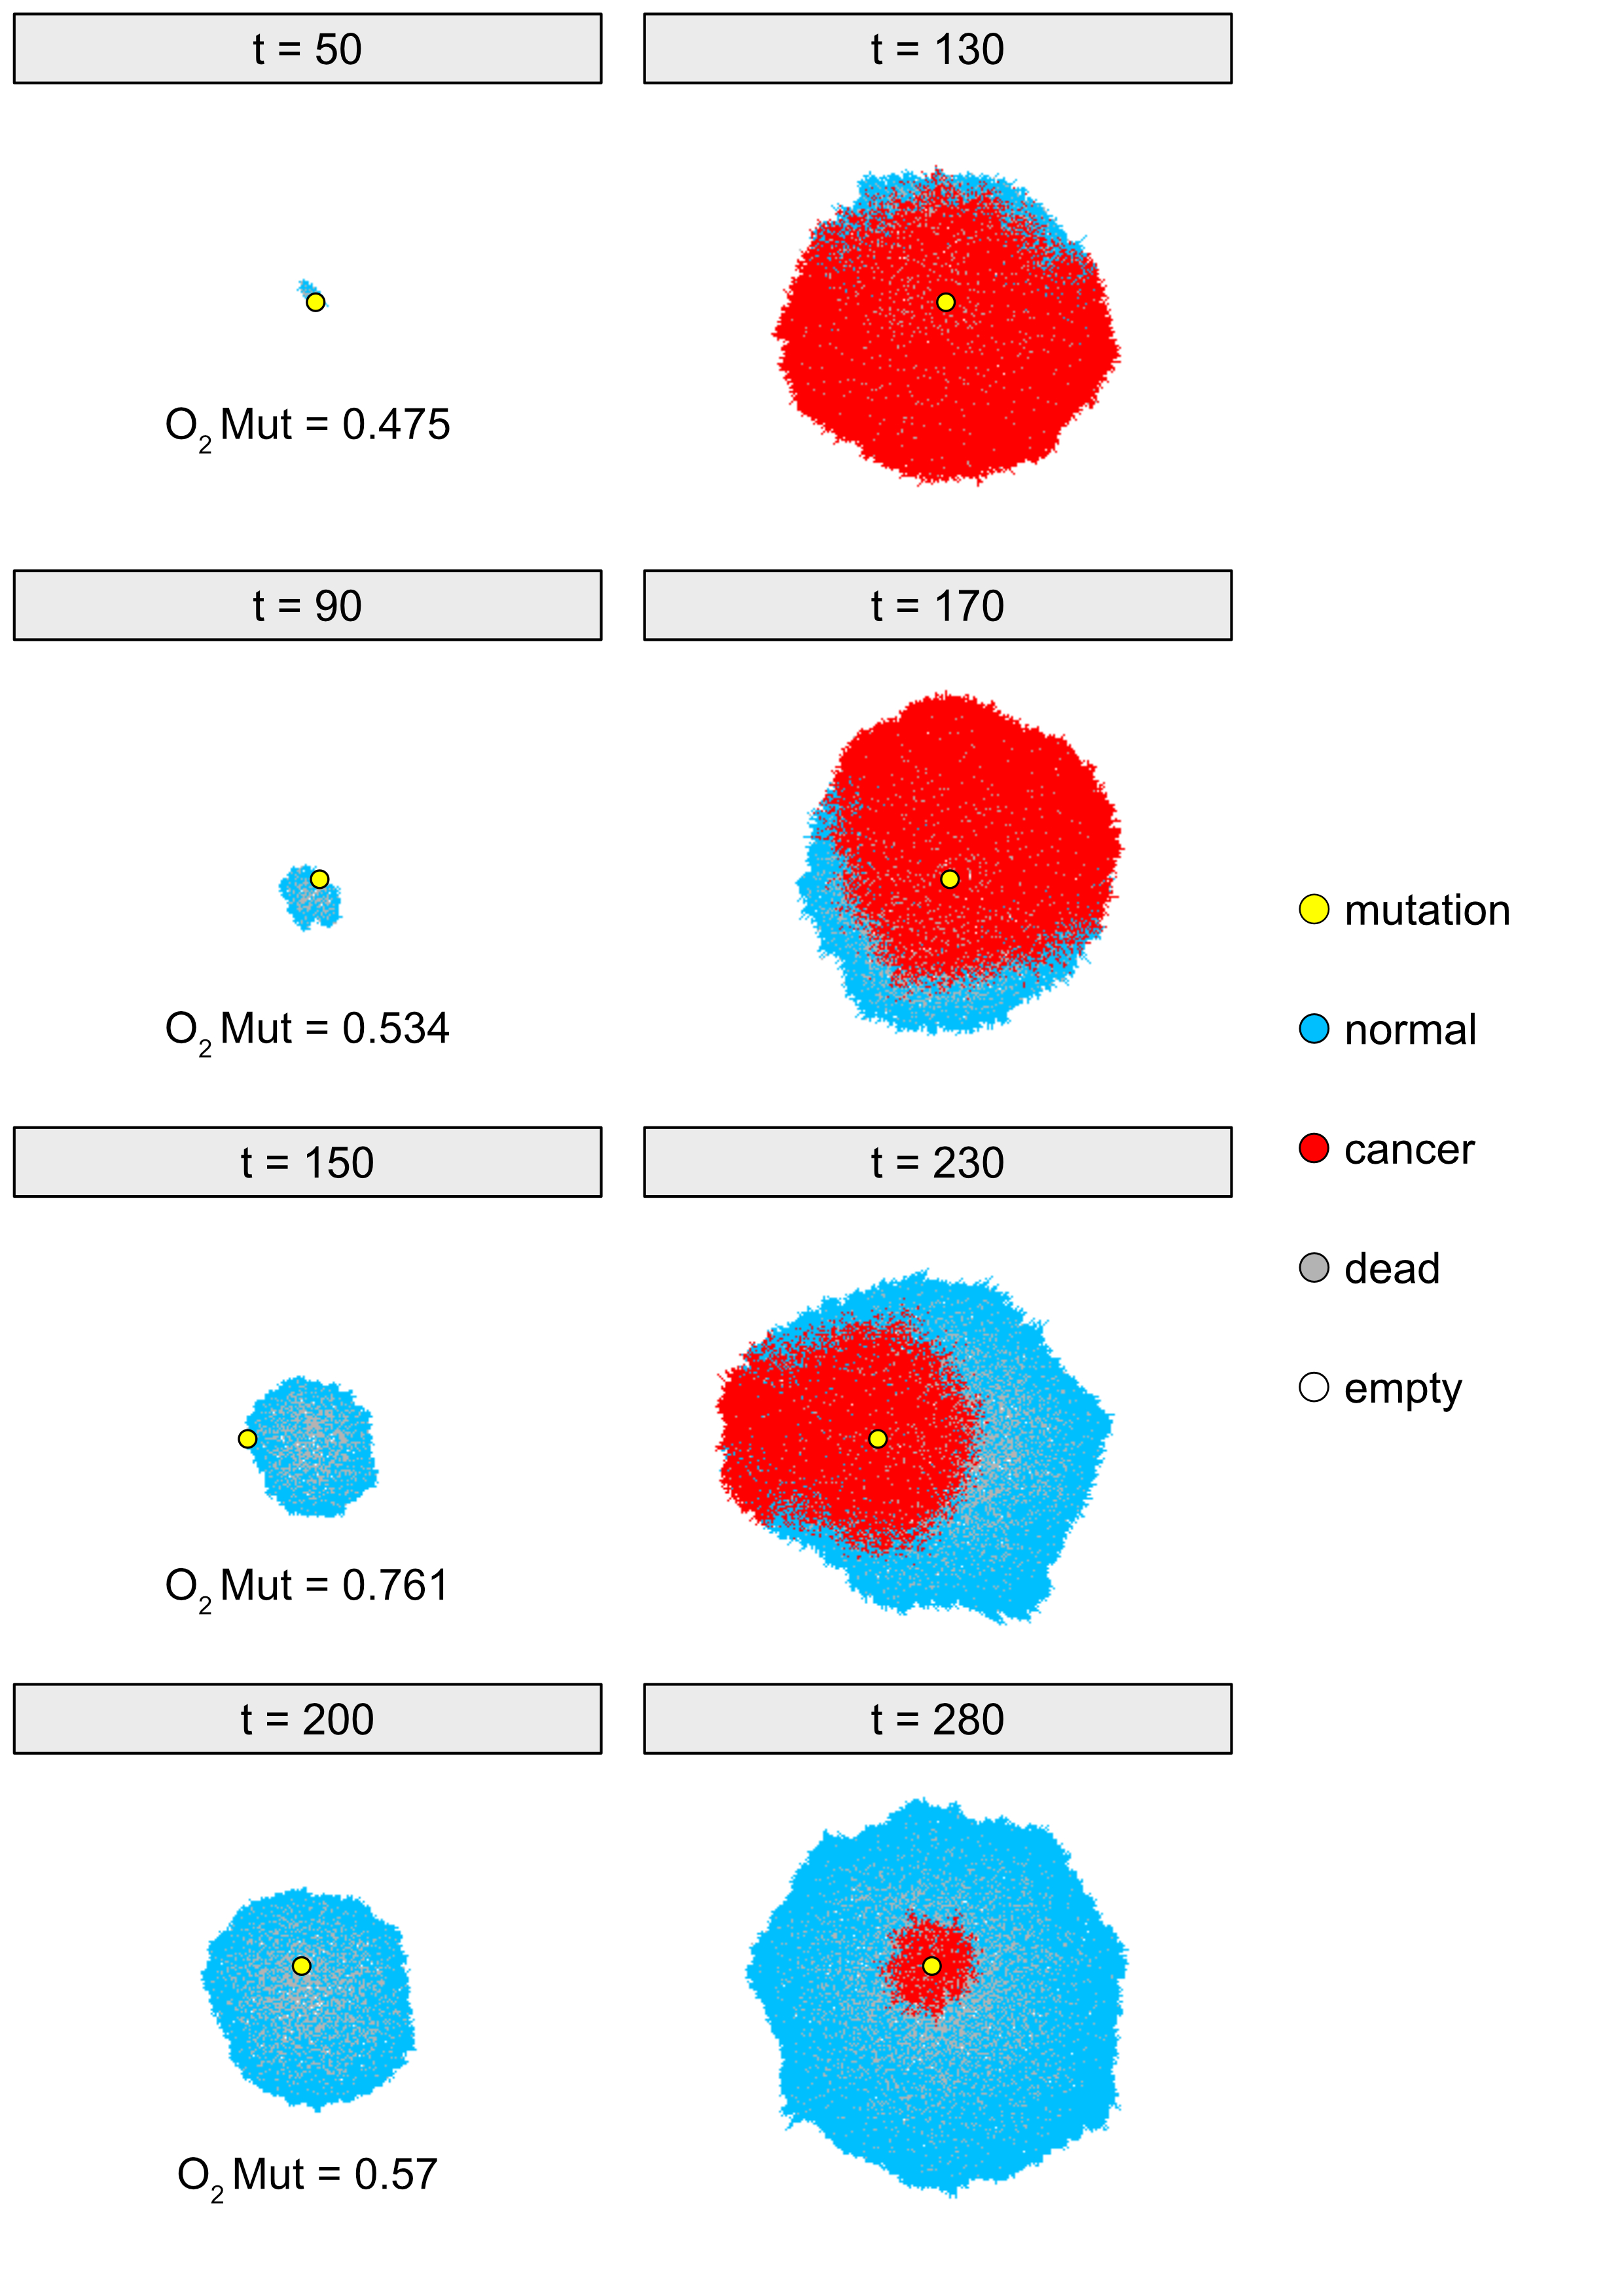
\includegraphics[width=0.9\textwidth]{Seed6_diff_t_mut.jpg}
  \caption{Agent-based lattice snapshots for  seed 6 illustrating the impact of the mutation event on tumor growth.
Left panels show the lattice configuration at the time the mutation is introduced, 
while right panels show the corresponding configurations after a fixed interval of 80 time steps following the mutation.
$t$ denotes simulation time, the yellow circle marks the mutation site, and $O_{2}^{\mathrm{mut}}$ denotes the local oxygen concentration at that site. }
  \label{fig:seed6}
\end{figure}



\newpage
\subsection{Effect of crowding on cells growth}
To investigate the role of stochasticity in tumor evolution, simulations were performed with a fixed mutation time for different seeds.
Figure~\ref{fig:seed6_seed10} shows representative lattice snapshots for seeds 6 and 10 at the mutation time
$t_{\mathrm{mut}} = 120$ (left column) and at a later time $t = 200$ (right column).

Even with the same mutation time, the outcomes differ strongly between seeds. In seed 10, the cancer population expands 
rapidly and occupies most of the lattice by $t=200$, whereas in seed 6 the cancer growth remains limited. This difference originates
from the stochastic placement of the mutation, which determines the local environment in which the first cancer cell appears. 

Further analysis shows that oxygen availability at the mutation site is not the main factor behind this behavior.
Instead, the key difference is the local density of normal cells at $t_{\mathrm{mut}}$. Quantifying this through
the number of normal cells $N_n(t,\mathrm{\text{seed number}})$, we find $N_n(t_{\mathrm{mut}}=120, 6)=1225$, compared to
$N_n(t_{\mathrm{mut}}=120, 10)=288$.
The much lower crowding in seed 10 allows the cancer population to expand more easily, especially given its higher
division and pushing probabilities and lower death probability compared to normal cells, as described earlier.


  
\begin{figure}[H]
  \centering
  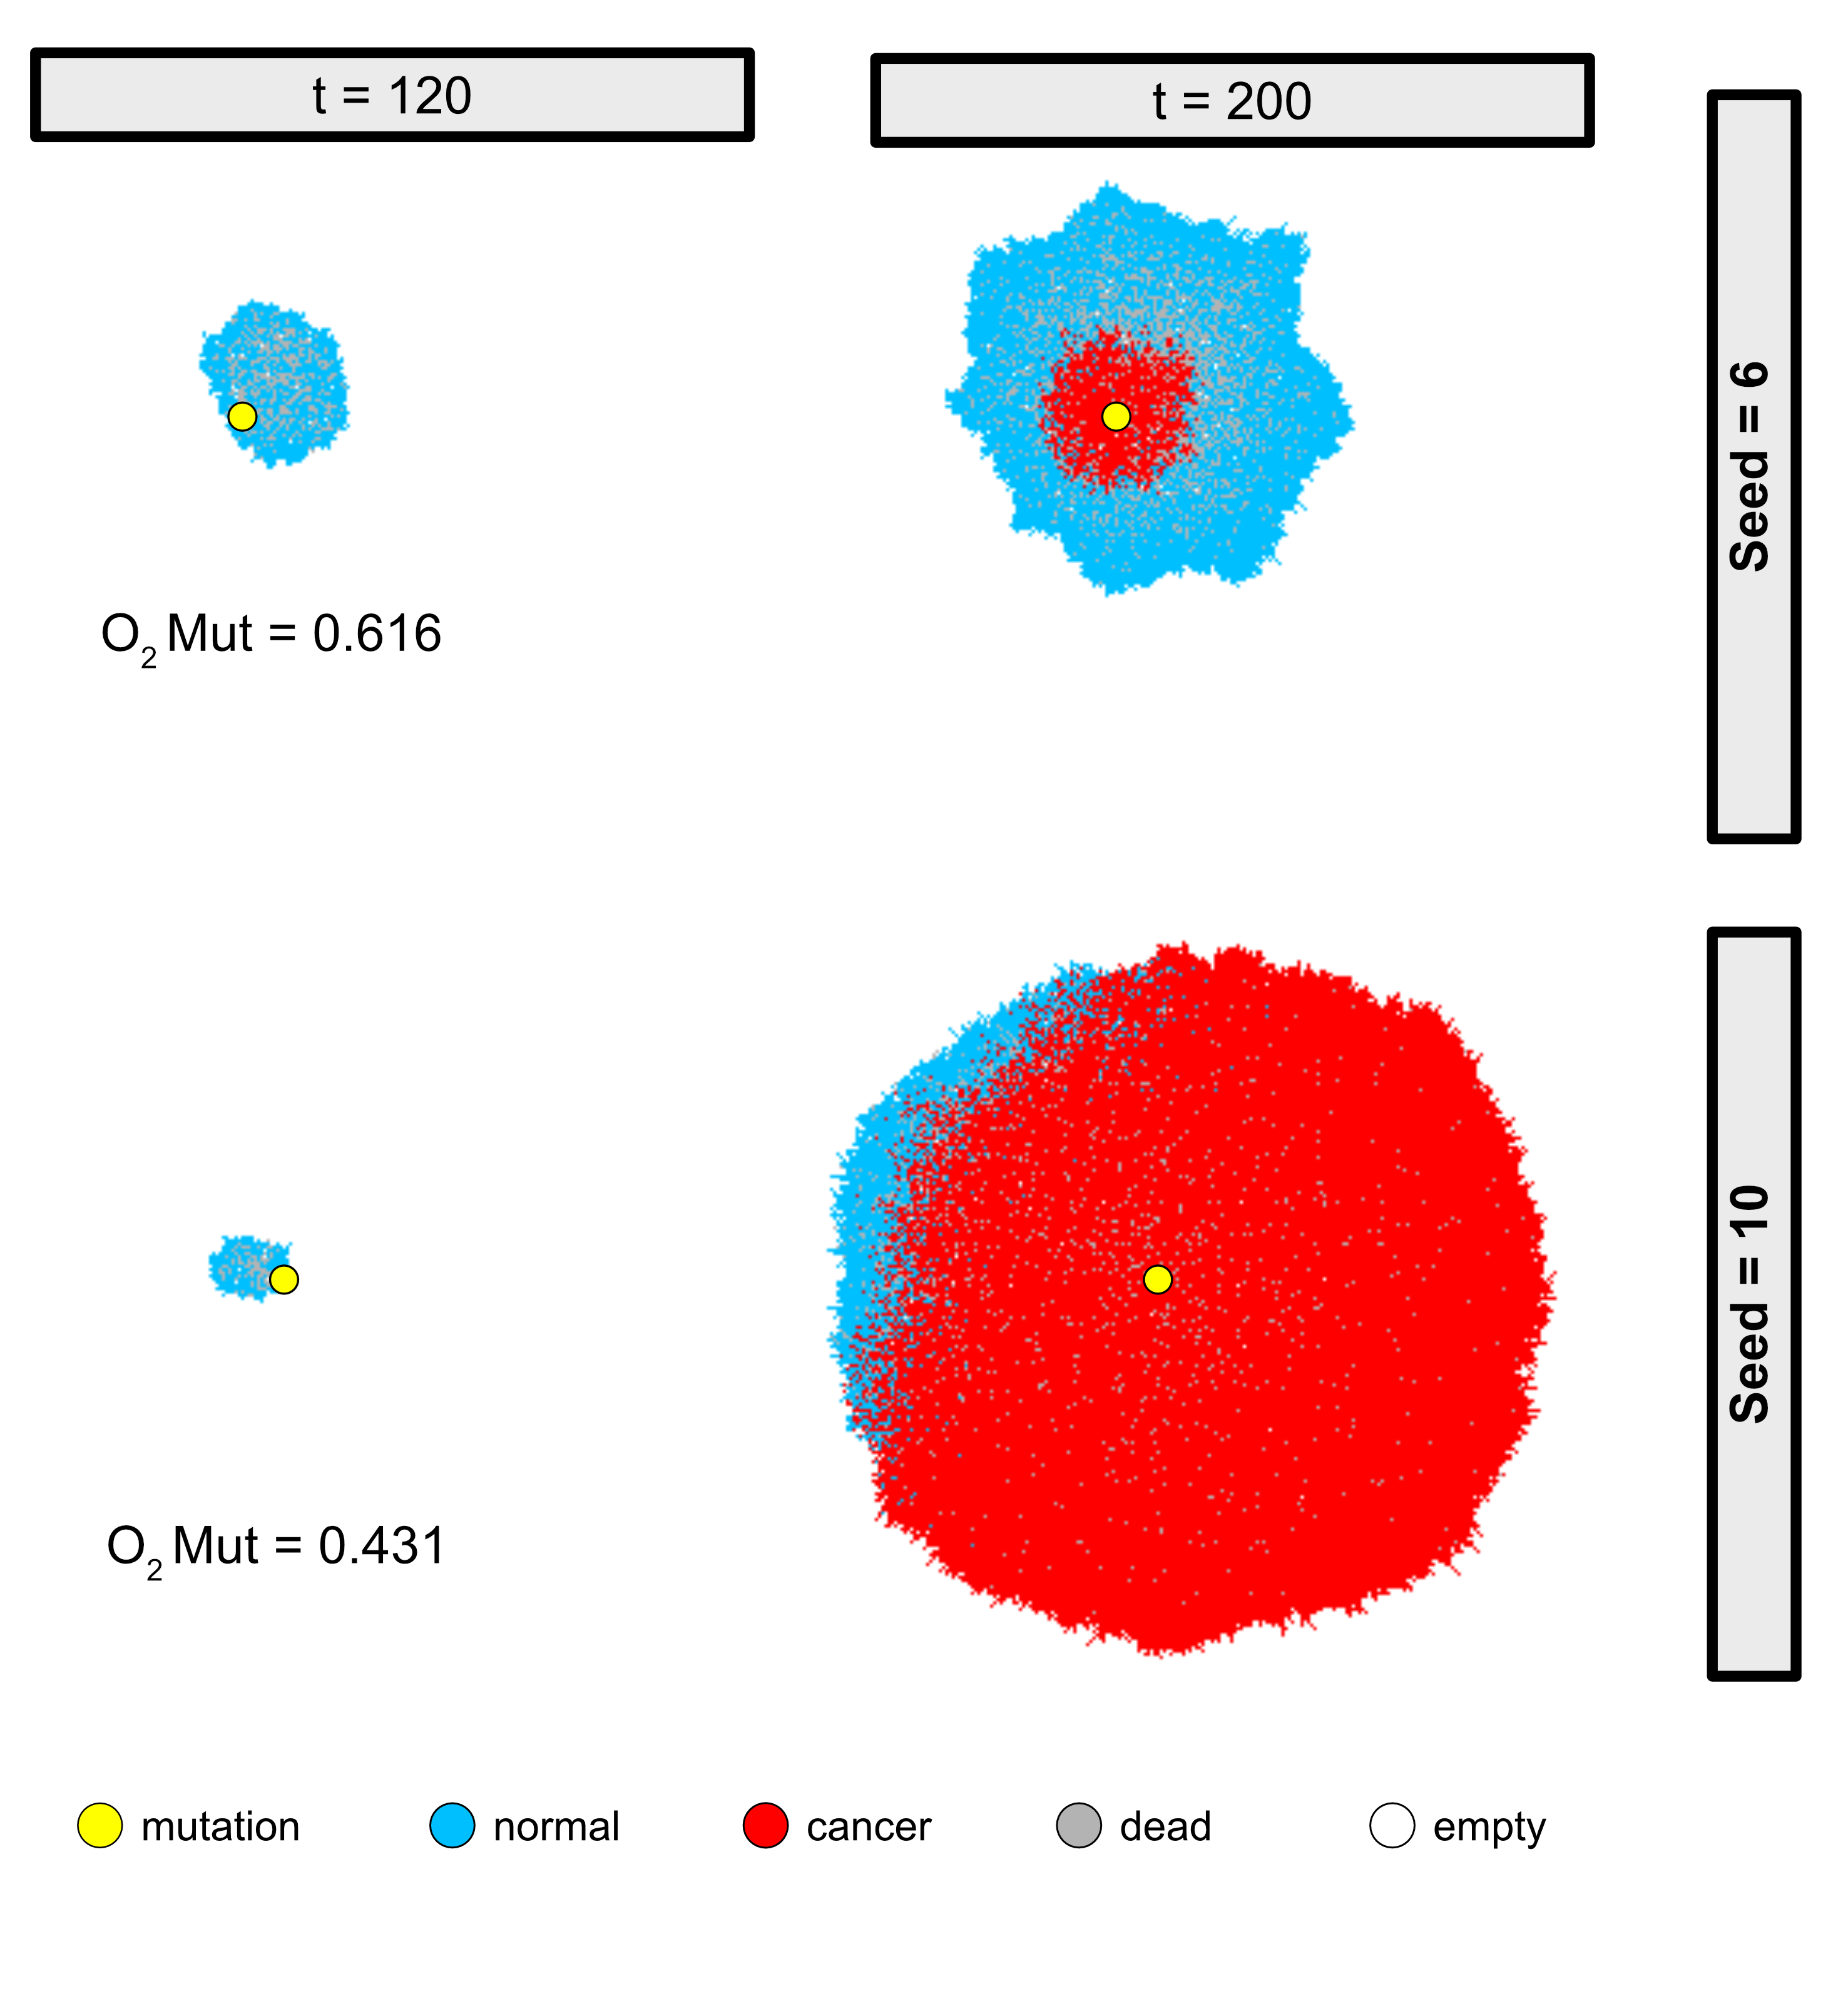
\includegraphics[width=0.6\textwidth]{seed6_seed10.jpg}
  \caption{Lattice snapshots for seeds 6 and 10 at the mutation time \(t_{\mathrm{mut}} = 120\) and at \(t = 200\).
The yellow circle marks the mutation site, and  $O_{2}^{\mathrm{mut}}$ denotes the local oxygen concentration at that location.}
  \label{fig:seed6_seed10}
\end{figure}


% ===============================
\section{Conclusion and Outlook}
% ===============================
In this work, we developed an agent-based lattice model to study tumor evolution within a growing normal cell population. 
As a proof of principle, the model was initially evaluated by testing different time points at which a cancerous mutation 
is introduced. As anticipated, when the mutation occurs at early time points during healthy cell population expansion, 
the higher division rate of cancer cells leads the mutant clone to rapidly expand and dominate the population. In contrast,
 when mutations are introduced at later time points, they arise within a large pre-existing healthy cell population, thereby
 limiting subsequent tumor clone expansion despite their higher division rate.

We next assessed the role of stochasticity by performing simulations with different random seeds while keeping the mutation
timing fixed. Intriguingly, different seeds resulted in distinct local conditions at the mutation site, leading to variations
in the number of normal cells present at the time of mutation. These differences directly influenced cancer expansion, 
highlighting the importance of local spatial crowding in determining tumor growth.

Overall, this project presents a simple and minimal modeling framework in which a limited number of key factors are integrated. 
The model yields tumor growth behaviors consistent with the expected influence of mutation timing and population composition. 
Future work could extend this framework by incorporating additional biological processes, such as multiple mutations, heterogeneous
 cell properties, and further microenvironmental factors, to study more complex tumor dynamics. In the current implementation, 
environmental factors such as oxygen are treated as a static diffusion-based background, and cellular oxygen consumption is
neglected for simplicity. For a more physiologically realistic setting, future extensions should incorporate dynamic oxygen uptake, 
nutrient availability, and related processes. Lastly, future work could enhance the model by integrating experimental data to fine-tune
model parameters, thereby improving its predictive capability.

\printbibliography

\end{document}
